\begin{appendices}

% \setcounter{algorithm}{0}
% \renewcommand\thealgorithm{A.\arabic{algorithm}}


\section{The Definition of Sensor Features}\label{apd:sen_features}

We explain the content of a sensor feature as mentioned in Section~\ref{sec:problem_formulation}.
At each timepoint $l$, the mobile sensor collects accelerometer readings $[x_l^{\mathfrak{L}},y_l^{\mathfrak{L}},z_l^{\mathfrak{L}}]$ and orientation readings $[x_l^{o},y_l^{o},z_l^{o},w_l^{o}]$. A graphic illustration of these sensor readings is shown in Figure~\ref{fig:frame_change}.
\begin{figure}[h]
    \centering
    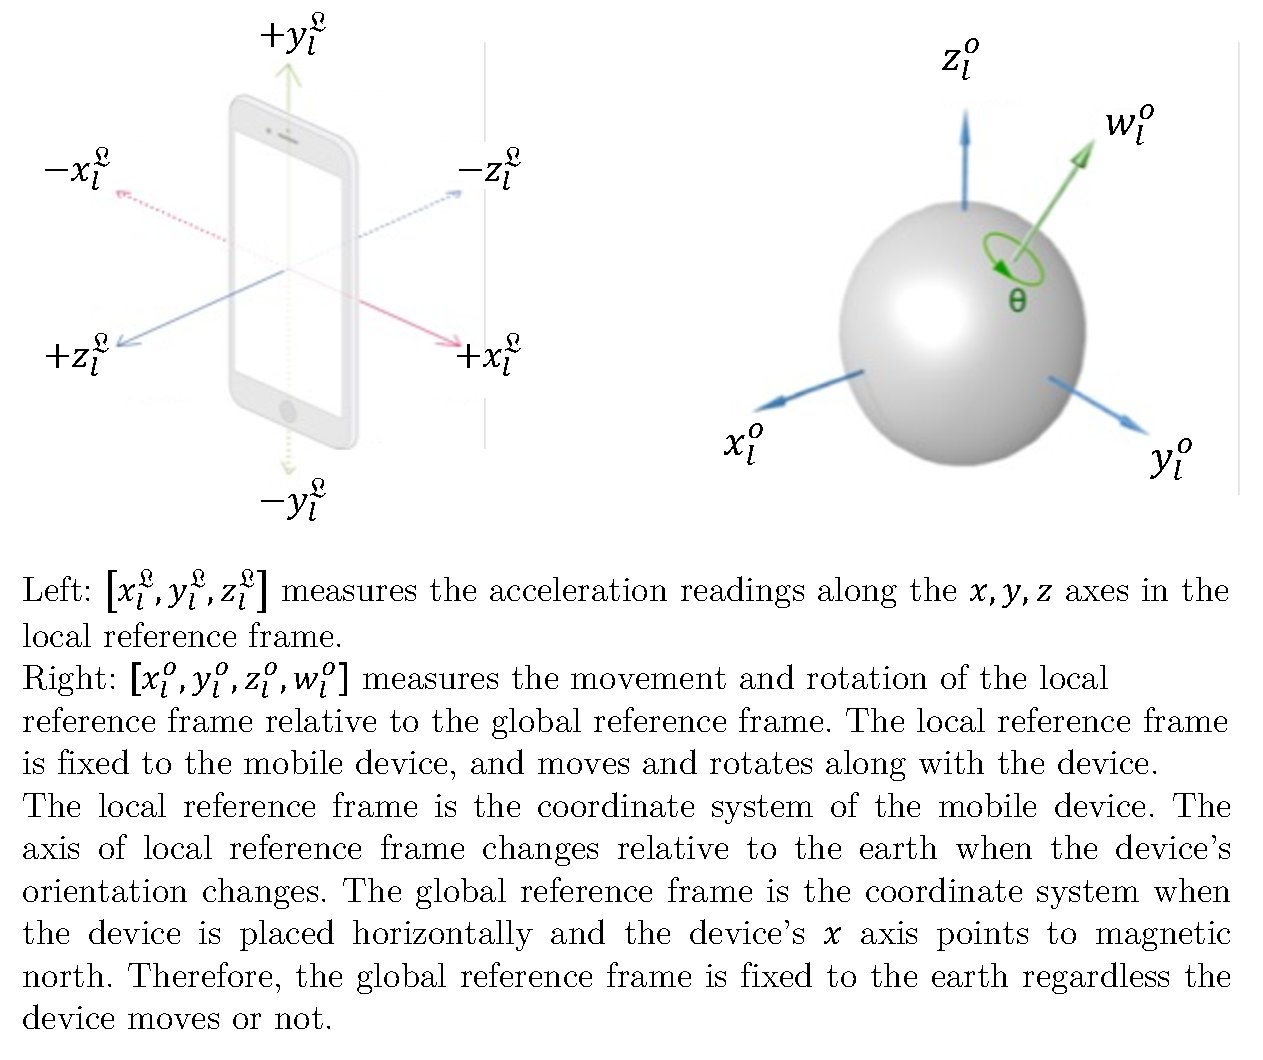
\includegraphics[width=0.7\textwidth]{imgs/frame_change.pdf}
    \caption{Sensor Readings \protect\cite{apple_inc_understanding_2022_a} }
    \label{fig:frame_change}
\end{figure}

The accelerometer readings are in the local reference frame, which most existing studies rely on \protect\cite{piau_when_2020_a,yu_wearable_2022_a,zhu_deep_2021_a}. However, these local reference readings do not reflect the precise walking pattern in the geographic coordinate system, because it moves and rotates along with the mobile device. To address this issue and make the interpretation more meaningful in the geographic sense, we decide to work with the readings in the global reference frame. We transform the local reference frame accelerometer vector $v_l^{\mathfrak{L}} =[x_l^{\mathfrak{L}},y_l^{\mathfrak{L}},z_l^{\mathfrak{L}}]^T$ to the global reference frame as $v_l^\mathfrak{G} =[x_l^{\mathfrak{G}},y_l^{\mathfrak{G}},z_l^{\mathfrak{G}}]^T$ via the quaternion rotation 
$$v_l^{\mathfrak{G}} = \mathcal{R}_l v_l^{\mathfrak{L}}$$ 
where $\mathcal{R}_l$ is the rotation matrix derived from quaternion $[x_l^{o},y_l^{o},z_l^{o},w_l^{o}]$ as follows. In general, given a quaternion $[x,y,z,w]$, the corresponding rotation matrix $\mathcal{R}$ is defined as\footnote{\url{https://en.wikipedia.org/wiki/Quaternions_and_spatial_rotation}}
\begin{equation}
\label{eq:rotation_matrix}
    \mathcal{R} = \begin{bmatrix}
        w^2+x^2-y^2-z^2 & 2 x y-2w z & 2 x z+2 w y \\  
        2 x y+2 w z & w^2-x^2+y^2-z^2 & 2 y z-2w x \\
        2 x z-2w y & 2 y z + 2 w x & w^2 - x^2- y^2 + z^2
    \end{bmatrix}.
\end{equation}
Then, we define the sensor feature $a_l$ as
\begin{equation}
a_{l}=[x_l^{\mathfrak{G}},y_l^{\mathfrak{G}},z_l^{\mathfrak{G}} ]^T.
\end{equation}

Following the best practice of data augmentation for mobile sensor data \citepsec{um_data_2017_a,zhang_deep_2020_a}, during the training stage, we further transform the input sensor features with random rotations to improve the generalization ability of our model. To do this, we first sample a quaternion using Algorithm \ref{alg:sample_quaternion} where $\text{Uniform}(b_1,b_2)$ means the uniform distribution on the interval $[b_1,b_2]$, and then plug the obtained quaternion into Equation \ref{eq:rotation_matrix} to construct a random rotation matrix. Within each training epoch and for each walking test, we construct a random rotation matrix $\tilde{\mathcal{R}}$ as described, and then use it to transform all sensor features of the walking test as $\langle \tilde{\mathcal{R}} a_1, \tilde{\mathcal{R}} a_2, \dots, \tilde{\mathcal{R}} a_L \rangle$. Once the training stage is finished, we use the original sensor features $\langle a_1, a_2, \dots, a_L \rangle$ to do inference.

\begin{algorithm}[h]
% \small
\caption{Sample a Quaternion}\label{alg:sample_quaternion}
\begin{algorithmic}[1]
\State Draw $x \sim \text{Uniform}(0,1)$, $y \sim \text{Uniform}(0,1)$, $z \sim \text{Uniform}(0,1)$.
\State Let $\text{norm}=\sqrt{x^2+y^2+z^2}$, and set $x=x/\text{norm}$, $y=y/\text{norm}$, $z=z/\text{norm}$.
\State Draw $\theta \sim \text{Uniform}(0,2\pi)$.
\State Set $w=\cos(\theta/2)$, $x=x \sin(\theta/2)$, $y=y \sin(\theta/2)$, $z=z \sin(\theta/2)$
\State Return $[x,y,z,w]$
\end{algorithmic}
\end{algorithm}

\clearpage

\section{The Specification of the Feature Extraction Layer}\label{apd:cnn}

Recall that $X_i$ denotes the sequence of sensor features of the $i$th walking test performed by a focal patient. In this section, we focus on extracting the feature matrix $H_i^\mathbb{S}$ from a single waling test, and therefore drop the subscript $i$ to simplify the notation. 
We partition $X$ into three segments according to in which task the sensor signals are recorded. Namely, $X=[X_{1}, X_{2}, X_{3}]$, which respectively denote the segment for the outbound, return, and rest (standing still) tasks. According to the definition of sensor features given in Appendix \ref{apd:sen_features}, each segment $X_j$ is in fact a matrix of size $3 \times L_j$ for $j=1,2,3$, where $L_j$ is the length of segment $j$. In general, different segments have different lengths in different walking tests. In what follows, we assume that $X$ has been downsampled with the frequency of 10 Hz, while the treatment of other sampling frequencies should be adjusted proportionally.

Under the sampling frequency of 10 Hz, we observe that the rest segment on average has the longest sequence, with $L_3=296$ by averaging over all walking tests. To facilitate batch training, we reshape each segment into a matrix of size $3 \times 300$, by either padding it with zero columns if its length is smaller than $300$, or discarding the extra columns if its length is larger than $300$.
After the reshaping step, we treat each segment $X_j$ as an input of $3$ channels and length $300$, and then use the same CNN layer to extract a feature matrix of size $128 \times 5$ from $X_j$. The CNN layer is composed by a sequence of one-dimensional convolution (Conv1d) layers, each followed in order by a one-dimensional batch normalization layer (BatchNorm1d), a max pooling layer (MaxPool1d), and lastly a leaky ReLU layer (LeakyReLU) with slope $0.01$ for non-linear activation \cite{goodfellow_deep_2016_a}. Following the style of \cite{zhu_deep_2021_a}, we report the detailed architecture of the CNN layer in Table \ref{tb:cnn_layer}. Since the BatchNorm1d layer and the LeakyReLU layer do not change the input shape, we do not list them in Table \ref{tb:cnn_layer}. After the last Conv1d layer in Table \ref{tb:cnn_layer}, we do not add the MaxPool1d layer nor the LeakyReLU layer.

\begin{table}[h]
\centering
\caption{The Specification of the CNN Layer}
\label{tb:cnn_layer}
\small
\begin{threeparttable}
\begin{tabular}{L{50pt}C{40pt}C{30pt}C{40pt}C{60pt}}
\toprule
% \midrule
    & Kernel Size & Stride & Output Channel & Output Shape \\ \midrule
    % Input & & & 3 & (3, 300) \\
    Conv1d & 8 & 1 & 256 & (256, 293) \\
    MaxPool1d & 2 & 2 & & (256, 146) \\
    
    Conv1d & 8 & 1 & 512 & (512, 139) \\
    MaxPool1d & 2 & 2 & & (512, 69) \\
    
    Conv1d & 8 & 1 & 256 & (256, 62) \\
    MaxPool1d & 2 & 2 & & (256, 31) \\
    
    Conv1d & 8 & 1 & 128 & (128, 24) \\
    MaxPool1d & 2 & 2 & & (128, 12) \\
    
    Conv1d & 8 & 1 & 128 & (128, 5) \\
    \bottomrule
\end{tabular}
\end{threeparttable}
\end{table}

Given the input $X=[X_1,X_2,X_3]$, we feed each segment $X_j$ into the same CNN layer specified above, and obtain a feature matrix $H_j^\mathbb{S}$ of size $128 \times 5$ for $j=1,2,3$. We then horizontally concatenate these feature matrices to obtain the final feature matrix as $H^\mathbb{S}=[H_1^\mathbb{S}, H_2^\mathbb{S}, H_3^\mathbb{S}]$ of size $n_e \times n_o$, where $n_e=128$ and $n_o=15$.

\clearpage

\section{The Density Function of the Logistic-Normal Distribution}\label{apd:der_logistic_normal}

We employ the change of variables formula \citepsec{murphy_probabilistic_2022_a} to derive Equation \ref{eq:sigmoid_gauss_density}, which in general states that if a random vector $x \in R^{M}$ is mapped to another random vector $z \in R^{M}$ by an invertible
function $f$, i.e., $z=f(x)$, then the density function of $z$, denoted by $p_z(z)$, is related to the density function of $x$, denoted by $p_x(x)$, by the following relationship:
\begin{equation}
\label{eq:change_of_var}
p_z(z) = p_x\big( g(z) \big) \big| \det[J_g(z)] \big|
\end{equation}
where $g$ is the inverse function of $f$, $J_{g}(z) \in R^{M \times M}$ is the Jacobian matrix of $g$ evaluated at $z$, $\det [.]$ is the matrix determinant operator, and $|.|$ is the absolute value operator. 

In our case, $z=\sigma(x)$, which means that $f=\sigma$ and $g=\sigma^{-1}$. Using the fact that $\partial x_m/\partial z_m = 1 / (z_m(1-z_m))$, the corresponding Jacobian matrix can be computed as
\begin{equation}
% \label{eq:jacobian}
J_{g}(z) =  \begin{pmatrix}
    \frac{1}{z_1 (1-z_1)} & 0 & \dots & 0 \\
    0 & \frac{1}{z_2 (1-z_2)} & \dots & 0 \\
    \vdots & \vdots & \ddots & \vdots \\
    0 & 0 & \dots & \frac{1}{z_M (1-z_M)}
    \end{pmatrix},
\end{equation}
which is a diagonal matrix because $\sigma^{-1}$ has been element-wisely applied on $z$. Given that $0< z_m < 1$ for $m=1,2,\dots,M$, all the diagonal elements are positive, and thus we have 
\begin{equation}
\label{eq:jacobain_det}
    \big| \det[J_g(z)] \big|  = \frac{1}{\prod_{m=1}^{M} z_{m}(1-z_{m})}.
\end{equation}
Recall that $x \sim \mathcal{N}(\mu, \Sigma)$, then the corresponding density function is given by 
\begin{equation}
\label{eq:gauss_density}
p_x(x) = \frac {\exp \big(-\frac{1}{2}(x-\mu)^{T}{\Sigma}^{-1}(x-\mu) \big)}{ \sqrt{(2 \pi)^{M} \det[\Sigma] }}.
\end{equation}
Plugging Equation \ref{eq:jacobain_det} and \ref{eq:gauss_density} into Equation \ref{eq:change_of_var}, and setting $x=\sigma^{-1}(z)$, we obtain Equation \ref{eq:sigmoid_gauss_density}.

\clearpage

\section{Manually Crafted Features for Benchmarks}\label{apd:mannual_features}

Recall that given a walking test, we observe a sequence of sensor signals $\langle v_1^{\mathfrak{L}}, v_2^{\mathfrak{L}}, \dots, v_L^{\mathfrak{L}} \rangle$, where $v_l^{\mathfrak{L}}$ is the accelerometer readings recorded in the local reference frame at timepoint $l$, as explained in Appendix \ref{apd:sen_features}. To simplify notation, we drop the superscript $\mathfrak{L}$, and write $v_l=[v_{x,l},v_{y,l},v_{z,l}]^T$.
Following \cite{yu_wearable_2022_a}, we define the following features for each given walking test. 

\begin{table}[h]
\centering
\caption{Features for Conventional Machine Learning Models}
\label{tb:baseline_features}
\small
\begin{threeparttable}
\begin{tabular}{L{160pt}L{290pt}}
\toprule
% \midrule
    Feature Name & Formula \\ \midrule
    Mean x-axis values &  $u_{x} = \frac{1}{L} \sum_{l=1}^{L} v_{x,l}$ \\
    Mean y-axis values &  $u_{y} = \frac{1}{L} \sum_{l=1}^{L} v_{y,l}$ \\
    Mean z-axis values &  $u_{z} = \frac{1}{L} \sum_{l=1}^{L} v_{z,l}$ \\
    St. D. of x-axis values &  $\sigma_{x} = \sqrt{\frac{1}{L-1} \sum_{l=1}^{L} (v_{x,l} - u_{x} )^2 } $ \\
    St. D. of y-axis values &  $\sigma_{y} = \sqrt{\frac{1}{L-1} \sum_{l=1}^{L} (v_{y,l} - u_{y} )^2 } $ \\
    St. D. of z-axis values &  $\sigma_{z} = \sqrt{\frac{1}{L-1} \sum_{l=1}^{L} (v_{z,l} - u_{z} )^2 } $ \\
    Mean magnitude &  $u_{v} = \frac{1}{L} \sum_{l=1}^{L} ||v_l||$, $||v_l||=\sqrt{v_{x,l}^2+v_{y,l}^2+v_{z,l}^2} $ \\
    St. D. of magnitude &  $\sigma_{v} = \sqrt{\frac{1}{L-1} \sum_{l=1}^{L} (||v_l|| - u_v)^2 } $ \\
    Mean x-axis jerk & $\alpha_{x} = \frac{1}{L-1} \sum_{l=1}^{L-1} d_{x,l}$, where $d_{x,l}=v_{x,l+1}-v_{x,l}$ \\
    Mean y-axis jerk & $\alpha_{y} = \frac{1}{L-1} \sum_{l=1}^{L-1} d_{y,l}$, where $d_{y,l}=v_{y,l+1}-v_{y,l}$  \\
    Mean z-axis jerk & $\alpha_{z} = \frac{1}{L-1} \sum_{l=1}^{L-1} d_{z,l}$, where $d_{z,l}=v_{z,l+1}-v_{z,l}$  \\
    St. D. of x-axis jerk &  $\beta_{x} = \sqrt{\frac{1}{L-2} \sum_{l=1}^{L-1} (d_{x,l} - \alpha_{x} )^2 } $ \\
    St. D. of y-axis jerk &  $\beta_{y} = \sqrt{\frac{1}{L-2} \sum_{l=1}^{L-1} (d_{y,l} - \alpha_{y} )^2 } $ \\
    St. D. of z-axis jerk &  $\beta_{z} = \sqrt{\frac{1}{L-2} \sum_{l=1}^{L-1} (d_{z,l} - \alpha_{z} )^2 } $ \\
    Mean jerk magnitude &  $\alpha_{d} = \frac{1}{L-1} \sum_{l=1}^{L-1} ||d_l|| $, where $||d_l||=\sqrt{d_{x,l}^2+d_{y,l}^2+d_{z,l}^2}$ \\
    St. D. of jerk magnitude & $\beta_{d} = \sqrt{\frac{1}{L-2} \sum_{l=1}^{L-1} (||d_l|| - \alpha_{d})^2 } $  \\
    Stride time variability on x-axis & \multicolumn{1}{p{290pt}}{
    (1) Identify signal peaks in x-axis, $[t_1,t_2,\dots,t_Q]$;\newline 
    (2) Identify stride times $[d t_1,d t_2,\dots,d t_{Q-1}]$, where $d t_i=t_{i+1}-t_i$; \newline 
    (3) Compute stride time variability $V_{x}=\sqrt{\frac{1}{Q-2} \sum_{i=1}^{Q-1} (d t_i - \overline{d t} )^2 }$ }  \\
    Stride time variability on y-axis & \multicolumn{1}{p{290pt}}{
    (1) Identify signal peaks in y-axis, $[t_1,t_2,\dots,t_Q]$;\newline 
    (2) Identify stride times $[d t_1,d t_2,\dots,d t_{Q-1}]$, where $d t_i=t_{i+1}-t_i$; \newline 
    (3) Compute stride time variability $V_{y}=\sqrt{\frac{1}{Q-2} \sum_{i=1}^{Q-1} (d t_i - \overline{d t} )^2 }$ }  \\
    Stride time variability on z-axis & \multicolumn{1}{p{290pt}}{
    (1) Identify signal peaks in z-axis, $[t_1,t_2,\dots,t_Q]$;\newline 
    (2) Identify stride times $[d t_1,d t_2,\dots,d t_{Q-1}]$, where $d t_i=t_{i+1}-t_i$; \newline 
    (3) Compute stride time variability $V_{z}=\sqrt{\frac{1}{Q-2} \sum_{i=1}^{Q-1} (d t_i - \overline{d t} )^2 }$ }  \\
    Stride time vairability on magnitude & \multicolumn{1}{p{290pt}}{
    (1) Identify signal peaks in magnitude, $[t_1,t_2,\dots,t_Q]$;\newline 
    (2) Identify stride times $[d t_1,d t_2,\dots,d t_{Q-1}]$, where $d t_i=t_{i+1}-t_i$; \newline 
    (3) Compute stride time variability $V_{v}=\sqrt{\frac{1}{Q-2} \sum_{i=1}^{Q-1} (d t_i - \overline{d t} )^2 }$ }  \\
    \bottomrule
\end{tabular}
\end{threeparttable}
\end{table}

\clearpage

\section{Factor Loadings of the Trust Scale}\label{apd:trust_factor_loading}

\begin{table}[h]
\centering
\caption{Factor Loadings of the Trust Scale}
\label{tb:factor_loading}
\small
\begin{threeparttable}
\begin{tabular}{L{60pt}C{60pt}}
\toprule
% \midrule
    Factor & Loading \\ \midrule
    Trust 1 & 0.533  \\
    Trust 2 & 0.993  \\
    Trust 3 & 0.759  \\
    Trust 4 &  0.620 \\
    Trust 5 &  0.805 \\
    Trust 6 & 0.798  \\
    Trust 7 &  0.946 \\
    Trust 8 &  0.933 \\
    Trust 9 &  0.932 \\
    \bottomrule
\end{tabular}
\end{threeparttable}
\end{table}

\clearpage


\bibliographystylesec{informs2014}
\bibliographysec{Project-IDDvSD-ap.bib} 


\end{appendices}